\section{Implementation}
In this section we will explain how we construct this simple solver in detail. First we will talk about the tool we use - ABC. We will briefly introduce the internal data structure and the API we used. Then we will show the circuit structure in AIG. Finally, we will illustrate the usage of ILP in the problem, the method to iteratively optimize the solution, and how to construct circuits to represent in-equations such as $a+b+c \geq 2$.
% 在這個段落會詳細講解我們如何建構這個簡單的Solver,首先介紹我們所使用的ABC package,裡面內建的部份資料結構以及可以使用的API;接下來因為我們會使用AIG的方式來儲存整個電路,所以會展示電路的架構圖;最後一部分使用ILP來達到iterative遞增解決問題的方式,簡單說明如何以電路設計類似$a+b+c \geq 2$的不等式。
\subsection{ABC Package}
ABC is a system for sequential synthesis and verification written by Berkeley Logic Synthesis and Verification Group. It combines scalable logic optimization based on And-Inverter Graphs (AIGs), optimal-delay DAG-based technology mapping for look-up tables and standard cells, and innovative algorithms for sequential synthesis and verification.
We mainly use command read\_verilog to read two verilog files, and construct the circuit referred to miter in ABC.
% ABC 是 A System for Sequential Synthesis and Verification 由 Berkely的Berkeley Logic Synthesis and Verification Group所建構,他可以用AIG的形式處理可擴張的電路,並且以DAG為基礎,最佳延遲為目標,在系統中運作時都會進行technology mapping。
% 我們主要使用read_verilog這個指令來有效的讀取兩個電路檔,並參考ABC中的miter與[9]來建構整個電路,

\subsection{AIG Structure}
And-inverter graph (AIG) is a directed, acyclic graph that represents a structural implementation of the logical functionality of a circuit or network.

Each AIG node represents an AND gate in the circuit, and each input pin can be inverted. Dealing with boolean satisfiability for formal verification with the AIG format has great advantages. The benefits also applies to model checking and equivalence checking.
After we read in the two files, we will immediately strash and let ABC automatically convert the network into AIG structures. Our circuit are shown in Fig. 1
    

In Fig. 1, the upper compartment is composed of n MUXes. Each MUX matches an output of Cir1, and the input value of the MUX will select one output from Cir2. The correspond Cir1 output and the selected output of Cir2 will be connected with an XOR gate. All XOR gates will then be connected to an OR gate to make sure all output matches are correct.

    \begin{figure}[H]
    \centering
    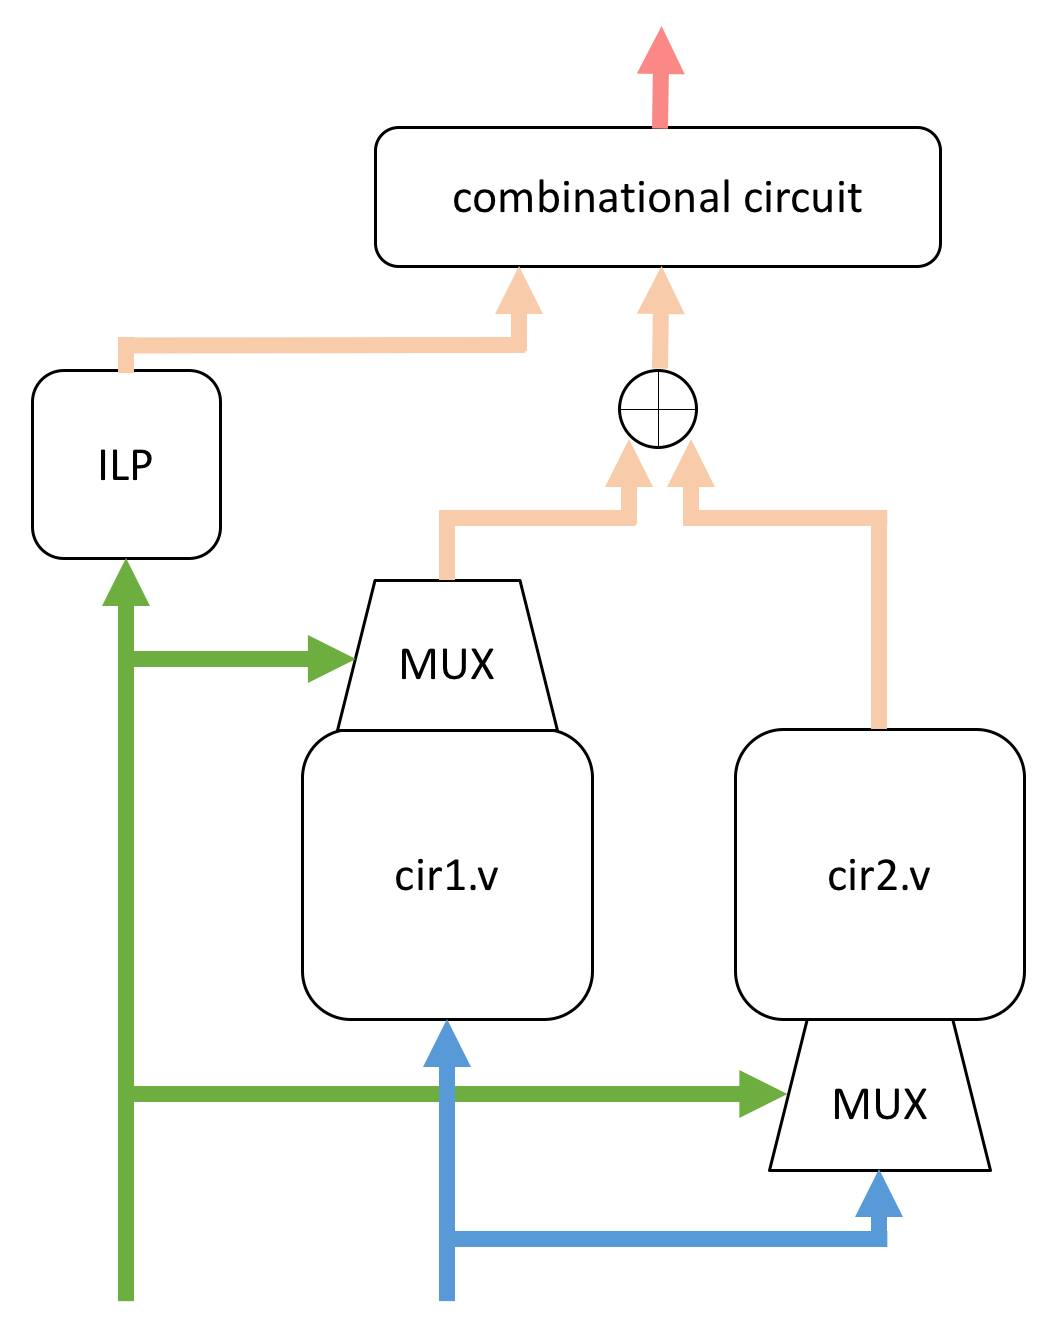
\includegraphics[scale=0.32]{images/structure}
    \caption{}
    \end{figure}

The similar logic applies to the lower compartment. Each MUX matches an input of Cir2, and the input value of the MUX will select one input from Cir1. The MUX will feed the correspond input of Cir1 into Cir2.
These two MUX groups simulate the matching process. By assigning values to each MUX groups, each assignments means one match pair patterns of the PI/POs. So the problem is simplified to assigning the input values of the MUXes, we just need to parse the values before output to generate the solution.
% 每一個AIG中的node代表一個電路圖中的And gate,並且在每一個input端可以決定這個值是否要被翻轉。以這種形式表示電路來處理Boolean satisfiability在formal verification的領域裡有非常大的成效,包含model checking以及equivalence checking。
% 因此在將兩個電路讀進ABC system後,進行strash的動作,直接將整個電路圖轉變成為AIG的形式以進行接下來的操作,如圖1所示。
% 放ppt的圖
\subsection{ILP Circuit}
 Note that we add an extra NULL bit for each output-side MUX. If the NULL bit is set, it means that the correspond output of Cir1 does not match with any Cir2 outputs.
To control the quality of our result, we connect all the NULL bits to an external ILP circuit to control the number of matching pairs. On one hand, if we set the minimum pairs to be 0 (which mean no restrictions at all), there is a possibility that the QBF solving will return an all NULL solution (no matching pair is also an answer); on the other hand, if we set the minimum pair number too high, it is likely we cannot find a single solution in the limited time. So we iteratively increase the minimum pair until the time limit hits. By doing so, we will at least have a decent solution before the time runs out.
% 在圖中,上半部份是由n個MUX所組成,每一個MUX會從Cir2的outputs裡面選一個作為輸出,輸出之後與Cir1中的每一個output連接至一個XOR gate,將所有的XOR的輸出連接至一個OR gate後,將控制輸出是否為CONST0的MUX連接至ILP circuit,最後將ILP的輸出與OR gate的輸出and在一起,得到最後的OUTPUT。

In Figure 2, each node of the graph is a MUX controlled by variable. If $a=1$ we choose 1, else we choose 0. For n variables and a constant k, the size of circuit is only $(n - k + 1)k$.
    
    \begin{figure}[H]
    \centering
    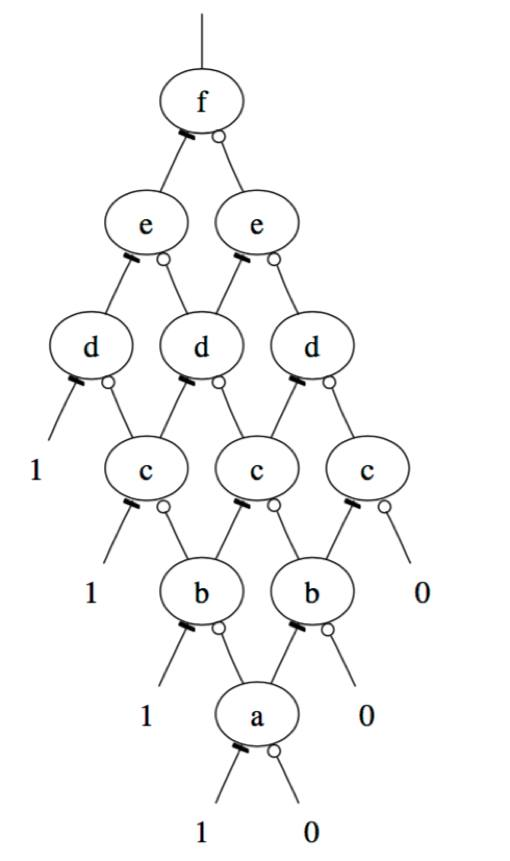
\includegraphics[scale=0.25]{images/ILP}
    \caption{ILP circuit for $a+b+c+d+e+f \geq 3$, from[6]}
    \end{figure}
